% \documentclass[a4paper,twoside]{article}
% \usepackage{fullpage}
% 
% 
% 
% 
% \usepackage[utf8]{inputenc}
% \usepackage[T1]{fontenc}
% \usepackage{RR}
% \usepackage{hyperref}
% 
% \usepackage{amssymb}
% \setcounter{tocdepth}{3}
% \usepackage{graphicx}
% 
% %%% Our Extra Packages %%%
% 
% %\usepackage{epic,eepic,amsmath,latexsym,amssymb,color,amsthm}
% \usepackage{ifthen}%,graphics,epsfig,fullpage} 
% 
% %%%
% 
% \usepackage{etoolbox}
% 
% 
% \usepackage{verbatim}
% \usepackage{graphicx}
% \usepackage{times}
% \usepackage{amsmath,amsfonts,amssymb,latexsym}
% %\usepackage{txfonts,pxfonts,wasysym}
% \usepackage{color}
% \usepackage{flushend}
% \usepackage{subfigure}
% \usepackage{multicol}
% \usepackage{hhline}
% \usepackage{cite}
% \usepackage[table]{xcolor}
% \usepackage{mathptmx}
% \usepackage{floatflt} 
% \usepackage{hyperref} 
% 
% 
% 
% 
% \usepackage{url}
% 
% 
% \newcommand{\ignore}[1]{}
% 
% %-----------------------for square--------------------------------------------
% \newlength {\squarewidth}
% \renewenvironment {square}
% {
% \setlength {\squarewidth} {\linewidth}
% \addtolength {\squarewidth} {-12pt}
% \renewcommand{\baselinestretch}{0.75} \footnotesize
% \begin {center}
% \begin {tabular} {|c|} \hline
% \begin {minipage} {\squarewidth}
% \medskip
% }{
% \end {minipage}
% \\ \hline
% \end{tabular}
% \end{center}
% }  
% %--------------------------------------------------------------------
% %--------------------------------------------------------------------
% %-------- macros for algorithm ---------------------------------------
% %\newtheorem{definition}{Definition}
% %\newtheorem{theorem}{Theorem}
% %\newtheorem{lemma}{Lemma}
% %\newtheorem{corollary}{Corollary}
% \newcommand{\toto}{xxx}
% %\newenvironment{proofT}{\noindent{\bf Proof }} {\hspace*{\fill}$\Box_{Theorem~\ref{\toto}}$\par\vspace{3mm}}
% %\newenvironment{proofL}{\noindent{\bf Proof }} {\hspace*{\fill}$\Box_{Lemma~\ref{\toto}}$\par\vspace{3mm}}
% %\newenvironment{proofC}{\noindent{\bf Proof }} {\hspace*{\fill}$\Box_{Corollary~\ref{\toto}}$\par\vspace{3mm}}
% 
% 
% \newcounter{linecounter}
% \newcommand{\linenumbering}{\ifthenelse{\value{linecounter}<10}{(0\arabic{linecounter})}{(\arabic{linecounter})}}
% \renewcommand{\line}[1]{\refstepcounter{linecounter}\label{#1}\linenumbering}
% \newcommand{\resetline}[1]{\setcounter{linecounter}{0}#1}
% \renewcommand{\thelinecounter}{\ifnum \value{linecounter} > 9\else 0\fi \arabic{linecounter}}
% 
% \newcommand{\tuple}[1]{\ensuremath{\left \langle #1 \right \rangle }}
% 
% %----------------------------------------------------------------------
% 
% 
% 
% 
% 
% 
% 
% %% d\'efinitions particulires  ce document %%%%%%%%%%%%%%%%%%%%%%%%%%%%%%%%%%
% % < mettre ici vos propres d\'efinitions \newcommand, \newenvironment, etc. > %
% %% fin des d\'efinitions particulires %%%%%%%%%%%%%%%%%%%%%%%%%%%%%%%%%%%%%%%%
% 
% 
% 
% \RRtitle{M\'emoire Transactionnelle: Imposer l'isolement forte entre transactions et op\'erations non-transactionnelle
% }
% 
% \RRetitle{ STM systems: Enforcing strong isolation between transactions and non-transactional code
% }
% 
% \RRauthor{         %% Le ou les auteurs %%%%%%%%%%%%%%%%%%%%%%%%%%%%%%%%%%%%
% \vspace{-1em}
% Tyler CRAIN\thanks[ur1]{IRISA, Universit\'e de Rennes 35042 Rennes Cedex, France}\and
% Eleni KANELLOU\thanksref{ur1}\and
% Michel RAYNAL\thanks{Institut Universitaire de France}\thanksref{ur1}
% \\
% {\it tyler.crain@irisa.fr, eleni.kanellou@irisa.fr, raynal@irisa.fr}
% }
% 
% 
% %% Champs pour les hauts de pages si diff\'erents du titre et des auteurs %%%%
% \authorhead{T. Crain, E. Kanellou \& M. Raynal}     %% auteurs : pages paires %%%%%%%%%%%%
% \titlehead{STM systems: Enforcing strong isolation between transactions and non-transactional code}      %% titre : pages impaires %%%%%%%%%%%%
% 
% \RRnote{         %% Note, contrat, collaboration, etc... %%%%%%%%%%%%%%%%%
% }
% 
% \RRdate{May 2012}         %% date de publication %%%%%%%%%%%%%%%%%%%%%%%%%%%%%%%%%%
%                    %% (si diff\'erente de la date systme %%%%%%%%%%%%%%%%%%%%
% 
% \RRNo{7970}           %% no du PI %%%%%%%%%%%%%%%%%%%%%%%%%%%%%%%%%%%%%%%%%%%%%
%                    %% (communique par le centre de doc )  %%%%%%%%%%%%%%%%%%
% 
% \RRresume{Ce rapport pr\'esente un algorithme de m\'emoire transactionnelle
% qui impose l'isolement forte entre transactions et op\'erations non-transactionnelle.
%         %% r\'esum\'e en franais %%%%%%%%%%%%%%%%%%%%%%%%%%%%%%%%%%%
% }                  %% fin du resume %%%%%%%%%%%%%%%%%%%%%%%%%%%%%%%%%%%%%%%%
% 
% \RRmotcle{m\'emoire transactionnelle, atomicité      %% Mots clef en franais %%%%%%%%%%%%%%%%%%%%%%%%%%%%%%%%
% }
% 
% \RRabstract{Transactional memory (TM) systems implement the concept of an atomic execution unit called  
% {\it transaction} in order to discharge programmers from explicit synchronization management. 
% But when shared data is atomically accessed by both transaction and non-transactional code, 
% a TM system must provide  {\it strong isolation} in order to overcome consistency problems.
% Strong isolation enforces ordering between non-transactional operations and transactions and 
% preserves the atomicity of a transaction even with respect to non-transactional code. 
% This paper presents a TM algorithm that implements strong isolation with the following features: 
% (a)  concurrency control of non-transactional operations is not based on locks and is particularly efficient, and 
% (b) any non-transactional read or write operation always terminates (there is no notion of commit\slash abort associated with them). 
%  %, TL2, Terminating Operation, Opacity, Non-transactional Operation, Consistency}   %% r\'esum\'e en anglais %%%%%%%%%%%%%%%%%%%%%%%%%%%%%%%%%%%%
% }                  %% fin de l'abstract %%%%%%%%%%%%%%%%%%%%%%%%%%%%%%%%%%%%
% 
% \RRkeyword{Transactional Memory, Strong Isolation, Atomicity       %% Mots clef en anglais %%%%%%%%%%%%%%%%%%%%%%%%%%%%%%%%%
% }
% \RRprojet{ASAP}
% \URRennes
% \RCRennes
% 
% 
% 
% 
% 
% \begin{document}
% 
% \makeRR

\section{Introduction}

By satisfying a consistency condition a concurrent protocol allows the
user of that protocl to reason about how that protocl will perform in
a concurrent setting.
For example a concurrent data structure that satisfies linearizability
means that the operations of a data strcuture will have a global order
base on real time.
This allows, for example, the programmer to use reasoning such as the follwing
when programming some network based service, if user $A$ who
is being serviced by thread $T_A$ changes his status to online (adding him
to the set of online users backed by a linearizable concurrent data structure)
then a query that is performed after the completion of the status change
on this set by user $B$ serviced by thread $T_B$ is guaranteed to contain
user $A$.
Without linearizability the programmer can use this reasoning, he might then
have to consider that the query by thread $T_B$ might or might not include $A$
leaving the programmer to have to come up with a solution for this.

Likewise in transactional memory, a correctness condition helps the
programmer reason about how he can use transactions in his programs.
For example opacity ensures that all transactions have a global order
and each transaction appears to have happened instantly at some point
in time between its invocation and commital.
This allows the programmer ....

At this point we will go back to the discussion of the previous chapter
on the difference between an operation on a concurrent object
and a transaction.
Let us try to motivate the difference by using an example.
For a concurrent object let us look at the common example of a tree
data structure implementing the set abstraction.
This abstraction might provide the following operations:
$insert(K)$ which adds $K$ to the set if it does not already exist, returning $true$
on success, $delete(K)$ which removes $K$, if it exists, from the set
returning $true$ on success, and $contains(K)$ returning $true$ if $K$
exists in the set.
There are two importnat things to notice, first is that these operations
are contained to their data structre implementation, the status of shared
memory outside of the data structure has no affect on these operations.
Second is that these operations fully implemnt the desired abstraction,
a user chooses to use this specific implementation because he needs
the $insert$, $delete$, and $contains$ operations.
If he wanted addtional functionality such as in-order iteration, then
he would have to choose a different implemntation providing the appropriate
abstraction.
In a way the data structure is a seperate entity from that of the program
created by the user where the user has access to this entity through
the interface given by the abstraction.

Transactions on the other hand are integreated into the users program
rather then compromising some seperate entity.
When a user places a trasaction in his code it is because he requires
synchronization between the processes of his program, this synchronization
does not have to be based on some predefined abstraction or only access
some contained structure.
The concept of the transaction allows the programmer to be free to
perform any sort of operation, performing reads and write to any
location in the shared memory.
In this sense the transaction is a different type of mechanism
then a concurrent object as transactions are contained within
a user's program instead of being separate entities behind
a fixed interface.

At a low level the difference between a transaction and an operation
on a shared object might imply certain protocol design chocies.
For example the previous chapter highlighted some of the implementation
differences between a traditional universal construction and a
universal construction for transaction based programs.
But before we consider implementation details we must consider how
the differences can be considered at an abstraction level.
Following the example of the previous chapter, this introduction
has expressed the view that transactions exsits as an integrated part of
a users program.
The pricipal concept of transactional memory is that within a transaction
the programmer calls $transaction\_read$ and $transaction\_write$ opertaions.
These operations are performed on the shared memory locations that a
programmer wants to access from within a transacion and the STM protocol
takes care of the difficult synchronization in order to ensure these opperations
appear as if they happen atomically.
At this point we have an important choice to consider dealing with the
shared memory that is accessed from within a transaction.
Should the shared memory that is accessed from within a transaction
be only safely accessable from within transactions, or should it be
safe to access memory inside and outside of transactions at any time,
or should it be something inbetween.
The follwoing section will discuss previous solutions on how to deal
with concurrent accesses to shared memory inside and outside of transactions,
followed by a discussion of where we think these solutions fall short
when considering ease-of-use before presenting a possible solution.

\subsection{Dealing with transactional and non-transactional memory accesses}

\paragraph{Strong vs Weak Isolation.}
TM has to guarantee that transactions will be isolated from each other, but
when it  comes to transactions and non-transactional  operations, there are
two  paths a  TM system  can follow:  it may  either act  oblivious  to the
concurrency between transactions and non-transactional 
operations, or  it may  take this concurrency  into account and  attempt to
provide     isolation    guarantees    even   between    transactional   and
non-transactional operations. The first  case is  referred to as \emph{weak
isolation} while the second case is referred to as \emph{strong  
isolation}.  (This  distinction  of   guarantees  was  originally  made  in
\cite{blundell06},  where   reference  was  made   to  {}``weak
atomicity'' versus {}``strong atomicity''.) 

While weak isolation  violates the isolation principle of
the  transaction abstraction, it could nevertheless be anticipated and used
appropriately by the  
programmer,  still resulting  in correctly  functioning  applications. This
would require the programmer 
to  be conscious  of  eventual race  conditions  between transactional  and
non-transactional code that can change depending on the STM system used.  


\paragraph{Desirable Properties.}
In order  to keep consistent with  the spirit of TM  principles, however, a
system should prevent unexpected   results  from   occurring  
in presence of  race conditions. 
Furthermore, concurrency   control should  ideally be implicit  
and never be delegated to  the programmer~\cite{CIR12,MS12}.  These are the  
reasons for  which strong isolation  is desirable. Under  strong isolation,
the aforementioned scenarios,   where non-transactional operations  violate
transaction isolation, would not be allowed to happen.  
An  intuitive approach  to  achieving  strong isolation  is  to treat  each
non-transactional operation that 
accesses shared data  as a ``mini-transaction'', i.e., one  that contains a
single operation. In that case,  transactions  will have to  be  
consistent (see Sect.~\ref{sec:badthings})  not only with 
respect to each other, but 
also with respect to the  non-transactional operations. However, while the
concept of the memory  transaction includes the possibility of abort,
the concept of the non-transactional operation does not.  This means that a
programmer expects  that a transaction  
might fail,  either by blocking or by  aborting. Non-transactional accesses
to shared data, though,  
will usually be  read or write operations, which  the programmer expects to
be  atomic. While executing, a  read  or write  operation   is  not 
expected  to  be de-scheduled, blocked or aborted.  



\paragraph{Content of the Paper.}
This paper presents  a TM  algorithm which takes the
previous issues into account. It is built on top of 
TM algorithm TL2 \cite{dice06},  a  word-based  TM algorithm  that  uses locks. 
More precisely,  TL2 is modified to provide strong isolation with non-transactional read 
and write operations.  However,  
the algorithm  is designed  without the use  of locks  for non-transactional
code, in order to guarantee that their execution will always terminate.  
To achieve  this,    two    additional     functions are specified, which substitute 
%${\sf non\_transactional\_read()}$ and ${\sf non\_transactional\_write()}$,  
%which  the programmer  has to  use instead  of 
conventional  read  or write operations that have to be performed  outside  of  a  transaction.  
%The  possible ``bad  scenarios''  of  running
%transactional and non-transactional code in  
%the absence of strong isolation 
Possible violations of correctness under strong isolation are reviewed in Sect. 
\ref{sec:badthings}. The TL2 algorithm is described in Sect. \ref{sec:tl2}. 
Section \ref{sec:protocol} describes  the proposed algorithm that implements
strong isolation for TL2, while  
Sect. \ref{sec:conclusions}  concludes the paper by  summarizing the work
and examining possible applications.  





%=======================================================================
\section{Correctness and Strong Isolation}
\label{sec:badthings}

\paragraph{Consistency Issues.}

% \ignore{When it comes  to environments where shared memory  is 
% accessed exclusively through transactions, then most accepted  
% consistency   conditions    build   on   the idea of  {\it serializability}
% \cite{P79}, a condition first  established  for  the study  of  database  transactions.}

Commonly, consistency conditions for TM build on the concept of 
{\it serializability} \cite{P79}, a condition first  established  for  the 
study  of  database  transactions.

% \ignore{For a  concurrent
% execution of transactions to be serializable, it must be  
% possible to find a serialization for it, i.e., a legal sequential execution
% that is equivalent to it. }

A concurrent execution of transactions is serializable, 
if there exists a serialization, i.e., a legal sequential execution equivalent to it.
Serializability refers only to committed  transactions,  however, and fails to take into 
account the possible program exceptions that a TM transaction may cause - even if 
it aborts - when it observes an inconsistent state of memory.

% \ignore{  the  context of  memory transactions,  stricter
% criteria are desirable, because even transactions that  
% will  eventually abort  may cause  program  exceptions if  they observe  an
% inconsistent state of the shared memory.  For this  
% reason, a  prominent consistency condition for  transactional memory, which
% is stricter than serializability,  has been proposed. }

{\it Opacity} \cite{guerraoui08}, a stricter consistency condition for TM, 
requires   that  both committed as well as aborted transactions  
observe a  consistent state  of shared memory.  This implies that  in order  for a
concurrent execution of memory transactions to be  
opaque,  there must exist  an equivalent,  legal sequential  execution that
includes both committed transactions and aborted  
transactions, albeit reduced to their read prefix.  Other consistency conditions 
have also been proposed, such as {\it virtual world consistency}~\cite{IR09}. It is weaker than 
opacity while keeping its spirit (i.e., it depends on both committed 
transactions and aborted transactions). 

%\vspace{-0.2cm}

\paragraph{Transaction vs Non-transactional Code.}
In a  concurrent environment,  shared memory  may  occasionally be
accessed by both transactions as well as  
non-transactional operations. %This  is mostly brought about by  the need to
%continue using legacy code that existed before  
%transactional memory was  implemented. 
Traditionally, however, transactions
are designed to synchronize only with other transactions  
without considering the possibility of  non-transactional code;
a program that accesses the same shared memory both transactionally
and non-transactionally would be considered incorrect.
A TM system that implements opacity minimally guarantees consistency between transactional
accesses, however, consistency violations  may  still be  
possible  in the  presence  of concurrent  non-transactional
code.
Given this, it can still be acceptable to have concurrent environments  
that may be prone to some types  of violations, as is the case with systems
that provide weak isolation \cite{blundell06,shpeis07}.
Under weak isolation, transactional and non-transactional operations can be
concurrent, but the programmer has to be aware of how to handle these.
%Traditionally, the same goes for code that is non-transactional: It  
%is not expected from the  programmer to know the synchronization details of
%the transactional memory algorithm that will run  
%concurrently with  her non-transactional code.  
%Therefore, this possibility
%of {\it co-existence of two different paradigms}, as well as  
%the  fact that  transactional memory  is mostly  implemented as  a software
%platform - instead of the transaction abstraction being  
%directly  provided by  the hardware  -  reveal  two different  aspects that
%transactional memory may acquire: In the first aspect,  
%it  is  the  only way  through  which  shared  memory  may be  accessed  by
%concurrent processes.  In the second aspect, which  
%comes into view when it exists alongside non-transactional code, it is just
%another means of achieving synchronization,  
%along with  locks, fences  and other traditional methods.  
Interestingly, this possibility of {\it co-existence of two different paradigms}
between strong and weak isolation reveals 
two different interpretations of transactional memory: On one hand considering TM as an implementation
of shared memory, and, on the other hand, considering TM as an additional way of achieving synchronization, 
to be used alongside with locks, fences, and other traditional methods.

Under weak isolation, transactions are considered to  
happen atomically only  with respect to other transactions.  It is possible
for non-transactional operations to see intermediate results  
of transactions that are still  live. Conversely, a transaction may see the
results of non-transactional operations that happened during  
the  transaction{}'s   execution.  If  this  behavior   is  not  considered
acceptable for an application, then the responsibility to prevent it is  
delegated   to  the   programmer  of   concurrent  applications   for  this
system. However, in order to spare the programmer this responsibility,  
both the  transactional memory algorithm  as well as  the non-transactional
read and write operations must be implemented in a way  
that  takes their co-existence  into account.  Such an  implementation that
provides synchronization  between transactional and  non-transactional code
is said to provide strong isolation.  


\paragraph{Providing Strong Isolation.}

There  are different  definitions in  literature for  strong 
isolation \cite{blundell06,ma07,harris06}.
In this paper we consider strong isolation to be the following:
%\begin{enumerate}
%\vspace{-0.1cm}
%\item   Non-transactional   operations   are   considered   as ``mini''
%transactions which never abort and  contain only a single  read or 
%write operation. 
%\vspace{-0.2cm}
%\item The consistency condition for transactions is opacity.
%\end{enumerate}
%As non-transactional read an write operations never abort, 
%this is called {\it terminating strong isolation} in the following.
(a) non-transactional   operations   are   considered  as ``mini''
transactions which never abort and  contain only a single  read or 
write operation, and (b) the consistency condition for transactions is opacity.
 
This definition implies that the properties that are referred to  as  
{\it containment}  and {\it non-interference} \cite{blundell06} are satisfied.  
Containment is   illustrated in  the  left  part of  Fig.
\ref{fig:int-nonc}.  There,
under strong  isolation, we have  to assume that transaction  $T_1$ happens
atomically,  
i.e.,``all  or  nothing'',   also  with  respect  to  non-transactional
operations. Then, while $T_1$ is  alive, no non-transactional read, such as
$R_x$, should be  
able to obtain  the value written to $x$  by $T_1$. Non-interference
is  illustrated  in  the right part of Fig.  \ref{fig:int-nonc}.  
Under  strong  isolation, non-transactional  
code   should  not  interfere   with  operations   that  happen   inside  a
transaction. Therefore, transaction $T_1$ should not be able to observe the
effects of  operations $W_x$ and $W_y$, given that they happen concurrently with it, 
while no opacity-preserving serialization of $T_1$, $W_x$ and $W_y$ can be found. 
Non-interference violations can be caused, for example,  by non-transactional 
operations that are such as to cause the ABA problem for a transaction that has 
read a shared variable $x$.
% Non-interference of  a transaction  $T_1$ can also  
% be compromised  by the interaction between non-transactional  operations  and  
% another  transaction   $T_2$. 
An additional feature of strong isolation, implemented in this paper, 
is that non-transactional read and write operations never block or abort. 
For this reason, it is termed {\it terminating strong isolation}.

\begin{figure*}[ht]
\centerline{
     \mbox{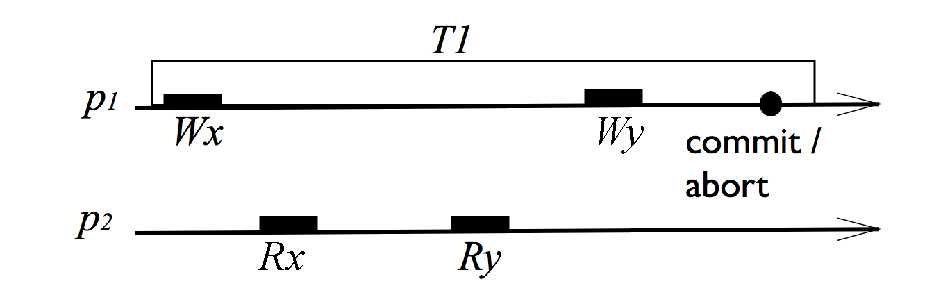
\includegraphics[width=0.4\textwidth]{SI/imgs/non_containment}}     
		%\mbox{\fig{file=imgs/non_containment, width=0.5\textwidth, clip=}}
    \mbox{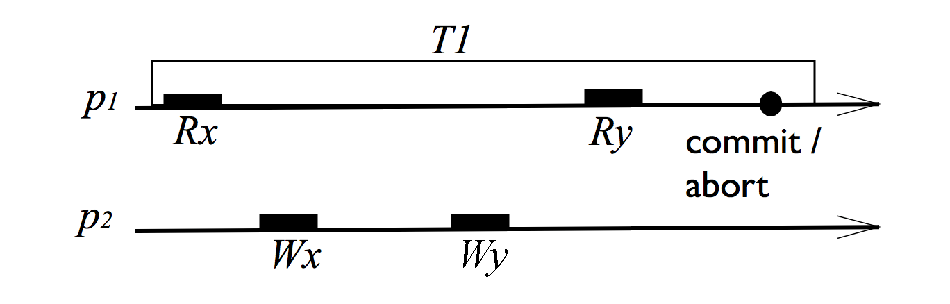
\includegraphics[width=0.4\textwidth]{SI/imgs/interference}}
		%\mbox{\fig{file=imgs/interference, width=0.5\textwidth, clip=}}
}
\caption{Left:  {\it Containment}  (operation $R_x$  should not  return the
    value written to $x$ inside the transaction). 
Right:  {\it  Non-Interference} (wile  it is still  executing, transaction
$T_1$ should not have access to the values that were written to $x$ and $y$
by process $p_2$).} 
\label{fig:int-nonc}
\end{figure*}
%An additional feature of strong isolation, implemented in this paper, 
%is that non-transactional read and write operations never abort. 
%For this reason, it is termed {\it terminating strong isolation}.


%Consider the
%case where a transaction $T$  
%pertaining  to process  $p_1$  reads variable  $x$  through read  operation
%$R_x$, and finds that it contains value  
%$v_1$.  Before $T$  commits, and  after  $R_x$ has  completed, assume  that
%another process $p_2$ modifies $x$  
%by  writing value  $v_2$ to  it through  non-transactional  write operation
%$W_{1x}$. Then, assume that either the  
%same process  $p_2$ or a different process  $p_3$ write non-transactionally
%value $v_1$ to $x$ through operation  
%$W_{2x}$. In  this case, process  $p1$ should have  a means to  detect this
%occurrence and transaction $T$ should  
%not commit, given that otherwise, strong isolation would be violated. 


%Non-interference for  a transaction  $T_1$ can also  be compromised  by 
%interaction between non-transactional  
%operations  and  another  transaction   $T_2$,  as  illustrated  in  Fig.
%\ref{fig:timent}. There, non-transactional operation  
%$R_{2x}$  reads  what transaction  $T_2$  has  written  to shared  variable
%$x$. Due to maintaining consistency, it is not  
%possible  to find  a  correct serialization  order where  non-transactional
%operation $W_y$ does not happen during the  
%duration  of transaction $T_1$,  violating non-interference.  Therefore, in
%order to preserve opacity, this situation would  
%have to  be detected when  transaction $T_1$ attempts to  execute operation
%$R_y$ and $T_1$ would have to be aborted. 
 

%\begin{figure*}[ht]
%\centerline{
%    \mbox{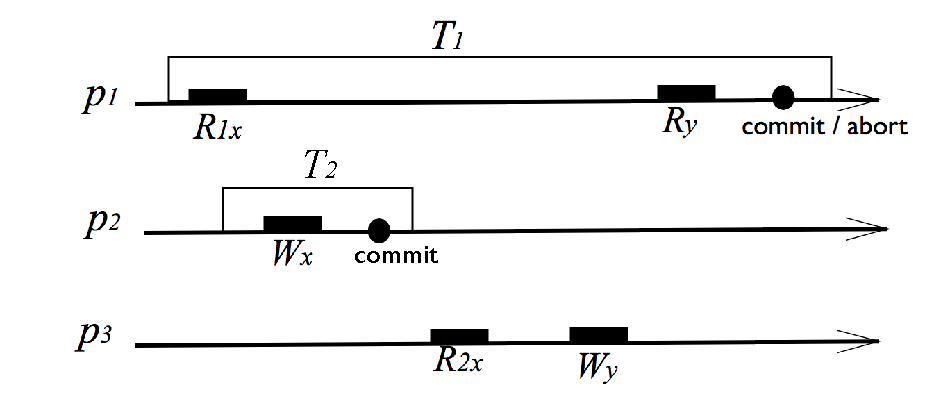
\includegraphics[width=0.5\textwidth]{imgs/time_NT.eps}}
%}
%\caption{Transaction  $T_2$  and  non-transactional operations  of  process
%$p_3$ interfere with transaction $T_1$.} 
%\label{fig:timent}
%\end{figure*}


\paragraph{Privatization/Publication.}
%In  a  system  that  does  not  provide  strong  isolation,  unsynchronized
%concurrent access can occur between two processes on a memory  
%area that both  view as shared. However, it can also  occur on memory areas
%that one of the threads views as shared while the other  
%considers them to  be its private memory area. 
%Another area where synchronization between transactional and 
%non-transactional code is needed, is the referred to  as the
A discussion of the co-existence of transactional and non-transactional code 
would not be complete without mentioning the
{\it privatization problem}. An area of shared memory is privatized,  
when a process  that modified it makes it  inaccessible to other concurrent
processes\footnote{Conversely, a memory area is made public  
when it goes from being exclusively accessible by one process to being 
accessible by several processes \cite{spear08} . 
This is referred  to as the {\it publication problem} and the consistency 
issues that arise are analogous.} with the purpose being
that the process can then access
the memory without using synchronization operations \cite{spear07}.  
A typical  example of privatization would  be the manipulation  of a shared
linked list. The  removal of a node by a  transaction $T_i$, for private
use, through  non-transactional  code,  by  the process  that  invoked $T_i$,  
constitutes  privatization. Then, $T_i$  is called privatizing transaction. 
While the privatization is not visible to all processes, inconsistencies may arise, given 
that for $T_i${}'s process the node is private but for other processes, the node is 
still seen as shared. 
%As shown in \cite{spear07}, incorrect results due to
%privatization can occur regardless of the update policy  that a  transactional 
%memory algorithm implements. 
Several solutions have been proposed for the privatization problem 
%such as using visible reads, conventional means of 
%synchronization such as fences, sandboxing, partitioning by consensus 
such as \cite{scott07,afek10,dice10}. %}, the use of lock-free reference   counters   \cite{afek10}  or   
%by  using private transactions \cite{dice10}, to name a few. 
%As  an example, consider
%the cases that result when given two processes $p_1$ and   
%$p_2$ that privatize shared variable $x$:
%\begin{itemize}
%\vspace{-0.1cm}
%\item  
%The TM implementation  uses a  redo log.  Process $p_1$ privatizes  $x$ with
%privatizing transaction $t_1$ but stalls before committing $t_1$.  
%$p_2$ executes during this stall and will not see the effects of $t_1$. 
%$p_2$ proceeds to privatize $x$ itself and to access it through 
%non-transactional operations. The variable $x$  will still be accessed through 
%transaction $t_1$ when process $p_1$ resumes and the results of $p_2$'s 
%privatization will not be visible to it. 
%\vspace{-0.2cm}
%\item The TM implementation uses an undo log. As above, $p_2$ privatizes 
%$x$ but $p_1$ stalls before performing validation before attempting 
%to commit. In the meanwhile, $p_2$ executes, privatizes $x$ and commits. 
%Given that updates are done in-place, $p_2$ will observe the updates 
%performed by $t_1$. However, when $t_1$ resumes and attempts to commit, 
%its validation will fail and it will abort. $p_2$ will be left privately 
%accessing data that are no longer valid.
%\end{itemize}
A system that provides {\it strong isolation} has the advantage of
inherently also solving the privatization problem, because it inherently 
imposes synchronization between transactional and non-transactional code.
%Strong isolation always imposes synchronization between 
%transactional and non-transactional code that access memory areas that 
%are potentially shared, which means that a system that guarantees strong 
%isolation is inherently privatization safe.


%========================================================================
\section{A Brief Presentation of TL2}
\label{sec:tl2}

%This section presents the main  aspects of the  TM algorithm TL2  which  are  
%used by the proposed algorithm. TL2 has been introduced by Dice, Shalev and Shavit 
%in    2006    \cite{dice06} and does not allow for  non-transactional code.  We describe 
%here the word-based version of TL2. In this  version it is considered that shared  memory 
%is accessed in the granularity of  single  memory words.  
%For the sake of  clarity and without loss  of generality, the rest of the description  
%assumes that shared variables are the size of a  memory word. 
%Therefore, the operations issued by a transaction are simply read and write operations. 
%For the sake of brevity, implementation details of the algorithm are omitted.  

TL2, aspects of which are used in this paper, has been introduced by Dice, Shalev and Shavit in 2006 \cite{dice06}.
The word-based version of the algorithm is used, %which means that the shared variables accessed are memory 
%words and that the operations issued by a transaction are simply read and write operations. 
%For the sake of brevity, implementation details of the algorithm are omitted in the following description. 
where transactional reads and writes are to single memory words.
%\vspace{-0.25cm}
%---------------------------------------------------------------------
%\subsection{Main Features of TL2}
\paragraph{Main Features of TL2.} The shared variables  that a  transaction reads form its {\it read
set}, while the variables it updates form the {\it write set}. 
Read operations in TL2 are {\it invisible},  meaning  that when  a  transaction reads  a  shared 
variable,  there is no indication of the read to other transactions.  Write operations are  
{\it deferred}, meaning that  TL2 does not perform the updates  as soon as  it {}``encounters'' 
the shared  variables that  it has to write to. Instead, the 
updates it has to perform are logged into a local list (also called {\it redo log}) and   are  applied 
to the shared  memory only once the transaction is certain  to commit. 
Read-only transactions in TL2 are considered efficient, because they don{}'t need to maintain 
local copies of a read or write set  and because they need no final read set  validation in order to commit.
To control transaction synchronization, TL2 employs locks and logical dates. 
%The variables  that a  transaction has to read form its read
%set, while the variable it has to update, form its write set.  
%A  transaction  first  has to  obtain  the  locks  that correspond  to  the
%variables of its write set, before it can  
%update them.  Conversely, a  transaction has to  check the logical dates  of the
%variables in its read set, in  
%order to  ensure that  the values  it has read  correspond to  a consistent
%snapshot of shared memory.  


%\paragraph{Locks.}
%TL2 locks  are stored in  a shared lock  table. Each shared memory  word is
%mapped to a lock through a  
%hash function\footnote{The  hash function is one-to-many,  resulting in one
%lock covering several shared  
%memory locations. This  partitions the memory into  so-called stripes.}. A
%lock is a memory word where  
%one of the  bits acts as lock  bit, indicating whether the lock  is free or
%not. The rest of the bits form the  
%logical date field.  The logical date of the lock  also serves as the 
%logical date of the
%memory  locations that  the lock  maps to.  Whenever a  shared  variable is
%modified, its logical date is also updated. Due to the way the  
%logical dates are assigned, they increment monotonically. 


\paragraph{Locks and Logical Date.}
A lock is associated with each shared variable.  
When a transaction attempts to commit it  first  has to  obtain  the  locks  of the
variables of its write set, before it can  
update them.
Furthermore, a  transaction has to  check the logical dates  of the
variables in its read set in  
order to  ensure that  the values  it has read  correspond to  a consistent
snapshot of shared memory.  TL2 implements logical time as an integer counter denoted $\mathit{GVC}$.
%$\mathit{GVC}$ is incremented by update transactions when they attempt to commit. 
When a transaction starts it reads the current value of $\mathit{GVC}$ into local variable, $\mathit{rv}$. 
When a transaction attempts to commit, it performs an increment-and-fetch on $\mathit{GVC}$, and stores the 
return value in local variable $\mathit{wv}$ (which can be seen as a write version number  or a version timestamp). 
Should the transaction commit, it will assign its $\mathit{wv}$ as the new logical date of the shared variables in its write set. 
%Timestamping with logical dates facilitates read set validation for a transaction. 
%When the read set of a transaction is not valid,  the transaction  cannot commit. 
%The  read set of  a transaction $T_A$ will be  invalidated  if another,  concurrent 
%transaction $T_B$ modifies shared  variable $x$ and commits, after $T_A$  has 
%read $x$  but while $T_A$ is  still active. 
A transaction must abort if its read set is not valid.  
%In TL2, it  can be detected that a transaction{}'s read  set is valid if 
Its read set is valid if the logical date of every  item in the set is less than the transaction{}'s $\mathit{rv}$  value. 
If, on the  contrary, the logical date of a read set  item is larger than the $\mathit{rv}$ 
of the transaction,  then  a concurrent  transaction 
has updated this item, invalidating the read.
%has performed  an   increment-and-fetch    of   $\mathit{GVC}$,   updated   the item  and  
%committed,  by  writing  the  new $\mathit{GVC}$ value into the item{}'s  logical date field.

%\paragraph{Update vs Read-only Transactions.}
%A {\it read-only} transaction in TL2 consists  of a  begin phase and  an operation phase.  
%An {\it update}  transaction has an additional commit phase. In  an update transaction, 
%the operation phase will contain write operations to shared variables as well as possibly 
%read operations, while  in a  read-only transaction, it  will solely contain read  operations. 
%Read operations in TL2 are {\it invisible},  meaning  that when  a  transaction reads  a  shared 
%variable,  there is  no indication of that fact towards  other transactions.  Write operations are  
%{\it deferred}, meaning that  TL2 does not perform the updates  as soon as  it {}``encounters'' 
%the shared  variables that  it has to write to (i.e., during the operation  phase). Instead, the 
%updates it has to perform are logged into a local list (also called  redo log) and   are  applied 
%to the shared  memory only once the transaction is certain  to commit (i.e. which occurs  during the
%commit phase). 


%\paragraph{Logical Time.}
%TL2 implements logical time as an integer counter denoted $\mathit{GVC}$.
%It is incremented by update transactions when they attempt to commit. 
%When it starts up, a transaction reads the current value of $\mathit{GVC}$ into local variable, $\mathit{rv}$. 
%When a transaction attempts to commit, it performs an increment-and-fetch on $\mathit{GVC}$, and stores the 
%return value in local variable $\mathit{wv}$ (which can be seen as a write version number  or a version timestamp). 
%Should the transaction commit, it will assign its $\mathit{wv}$ as the new logical date of the shared variables in its write set. 

%Timestamping with logical dates facilitates read set validation for a transaction. 
%When the read set of a transaction is not valid,  the transaction  cannot commit. 
%The  read set of  a transaction $T_A$ will be  invalidated  if another,  concurrent 
%transaction $T_B$ modifies shared  variable $x$ and commits, after $T_A$  has 
%read $x$  but while $T_A$ is  still active. 
%In TL2, it  can be detected that a transaction{}'s read  set is valid if the logical date 
%of every  item on the read set is less than the transaction{}'s $\mathit{rv}$  value. 
%If, on the  contrary, the logical date of a read set  item is larger than the $\mathit{rv}$ 
%of the transaction,  then this  indicates that,  in the meanwhile,  a concurrent  transaction 
%has performed  an   increment-and-fetch    of   $\mathit{GVC}$,   updated   the item  and  
%committed,  by  writing  the  new $\mathit{GVC}$ value into the item{}'s  logical date field.



%========================================================================
%\subsection{Inside a TL2 Transaction}
%\subsection{TL2 Read and Write Operations}
%\paragraph{TL2 Read and Write Operations}
%\paragraph{Begin of a Transaction.}
%When a  transaction starts  up, it  reads the current  value of  the $\mathit{GVC}$ 
%and stores it into  its local  $\mathit{rv}$ variable. %A transaction  has to keep  track of the
%variables in its read set and their  versions, as well as the variables in  its write set and 
%values that it has to write to them. Therefore, it  implements the  read and  write set  as 
%local lists,  which will  be filled during the transaction execution.  
%These data structures are also initialized at start-up.
%\begin{itemize}
%\paragraph{TL2 Write Operation.}
%\item When a transaction  has to update shared variable $x$, % it creates an entry
%for it in its local write set list  
%and there, it  stores $x${}'s address and the value that  has to be written to it.  
%it performs the intended update on the variable{}'s local copy in the transaction{}'s 
%redo log. If the transaction commits, the update will be performed during the commit phase.

%\paragraph{TL2 Read Operation.}
%\item When  a transaction has  to read  shared variable  $x$, then,  if it  is an
%update transaction, it first explores  its redo log in order to check whether $x$ is already contained
%there. Should this be the case,  then, in order to preserve consistency,  the value that is contained in the
%write set list will be returned for  the variable.  Otherwise, or in case it is read-only, a transaction checks 
%the lock and logical date of $x$ before and after reading it. If these checks determine that $x$ is not 
%concurrently updated by another transaction and reading it doesn{}'t invalidate the read set, the transaction 
%proceeds. Otherwise it aborts. 
%\end{itemize}
%Before and after reading $x${}'s value, a read-only transaction samples the
%lock bit and the lock version  
%corresponding to $x$. If the lock version is different before and after the
%read or if the lock bit is set, then  
%the transaction aborts, given that it has just detected a concurrent update
%of $x$ which invalidates its read  
%set.  If this  procedure, also  referred  to as  post-validation, does  not
%result in aborting, then the operation can   
%return the value that it has read  for $x$. If the transaction is an update
%transaction, then, before returning the  
%value, it  creates an entry for  $x$ in its  local read set list,  where it
%stores the memory address of $x$.  

%\paragraph{Attempt to Commit.}
%After  having executed  all its  read and/or  write operations, a transaction attempts  
%to commit. If  it is a read-only transaction, it has a consistent read set already and 
%commits without further explicit action. An update  transaction has to explicitly verify 
%whether it can commit by checking if it{}'s read set is still consistent. Then, in order 
%to make its updates  visible  to  the rest  of  transactions, it has to obtain the locks of 
%all variables in its write set and then update their values and their logical timestamps. 
%The logical timestamp is updated to the value of $wv$, which in turn is obtained by 
%performing an  increment-and-fetch  on $\mathit{GVC}$. The transaction commits 
%by releasing the locks again.


%\paragraph{Lock Acquisition and $\mathit{GVC}$ Increment.} 
%For  every item  in  the  transaction{}'s write  set,  bounded spinning  is
%performed on the corresponding lock in order  
%to  obtain  it.  If the  lock  acquisition  for  an  item fails,  then  the
%transaction aborts. If, however, all locks are acquired  
%successfully,   then  the   transaction  performs   increment-and-fetch  on
%$\mathit{GVC}$ and stores the return value in  
%local variable $\mathit{wv}$. This value of $\mathit{wv}$ will be stored as
%the new version of the variables in the  
%transaction's write set, if the transaction does not abort.

%\paragraph{Validation of the Read Set.}
%In order  to determine whether the  transaction has to abort,  a final read
%set validation takes place. During this  
%validation, it  is verified  for all  items of the  read set  whether their
%current version is still less that the transaction's  
%read version, $\mathit{rv}$, as well as whether the items are not locked by
%a different transaction. If it is detected  
%that this is not the case  for any item, the transaction aborts. Otherwise,
%the transaction can perform the intended  
%updates. Read  set validation  is not necessary  in the special  case where
%$\mathit{rv}$+1 = $\mathit{wv}$, given  
%that this would  guarantee that no concurrent transaction  has executed and
%possibly modified items of the read   set in the meanwhile.

%\paragraph{Deferred Updates and Lock Release.}
%The   address  and   update  value   for  each   shared  variable   in  the
%transaction{}'s write set is stored in a corresponding  
%entry  in the  transaction{}'s local  write set  list. Therefore,  for each
%write set list entry, the update value is stored in the  
%corresponding memory address. The  locks are released by atomically writing
%the value of $\mathit{wv}$ to their lock  
%version field  while clearing the lock bit. 



%========================================================================
\section{Implementing Terminating Strong  Isolation}
\label{sec:protocol}

A possible  solution to  the problem of  ensuring isolation   in the
presence of  non-transactional code consists in using  locks: Each shared
variable would then  
be associated with a lock and both transactions as well as non-transactional 
operations would have to access the lock before accessing the variable.

Locks are already used  in TM algorithms - such as TL2  itself - where it is
however     assumed   that  shared   memory   is   only  accessed   through
transactions. The use  of locks  in a TM algorithm  entails blocking and may
even lead a process to starvation. However,  
it can be argued that  these characteristics are acceptable, given that the
programmer  accepts the fact that a  transaction has a duration and that it
may  even  fail: The  fact  that   there is  always  a  possibility that  a
transaction will abort means that the eventuality of  
failure to complete can be considered a part of the transaction concept.  

On  the contrary,  when it  comes to single read or  write accesses  to  a shared
variable, a  non-transactional operation is  understood  as an
event  that  happens   atomically  and   completes.  Unfortunately   strong
isolation  implemented with  locks  entails the blocking  
of non-transactional read and write operations and would not provide termination.

Given that this approach would be rather counter-intuitive for the 
programmer (as well as possibly detrimental for program efficiency), 
the   algorithm presented  in this  section  provides  a solution  for adding
strong isolation which is not based on locks for the execution 
of non-transactional  operations. This  algorithm builds on  the base  of TM
algorithm  TL2 and  extends it in  order to account for  non-transactional 
operations. While read   and write operations that appear inside a 
transaction follow the original TL2 algorithm rather closely (cheap read 
only transactions, commit-time locking, write-back), 
the proposed algorithm 
specifies non-transactional read and  write operations 
that are to be used 
by the programmer, substituting conventional
shared memory read and write operations. 
TM with strong isolation has also been proposed in
software \cite{SMSA08,shpeis07} in hardware \cite{MTCM07}, and has been suggested to be too costly \cite{DS09}.
This work differs from other implementations in that it is terminating and
is implemented on top of a state-of-the-art STM in order to avoid too much extra cost.


%===================================================================
\subsection{Memory Set-up and Data Structures.}


\paragraph{Memory Set-up.}
The underlying memory system is made up of atomic read/write registers. 
Moreover some of them can also be accessed by the the following two 
operations. The operation denoted 
${\sf Fetch\&increment}()$ atomically adds one to the register and 
returns its previous value. 
 The operation denoted 
${\sf C\&S}()$ (for compare and swap) is a conditional write. 
${\sf C\&S}(x,a,b)$ writes $b$ into $x$ iff $x=a$. In that case it 
returns $\mathit{true}$. Otherwise it returns  $\mathit{false}$. 


The proposed algorithm assumes that the
variables  are  of  types and  values  that  can  be   stored in  a  memory
word. This assumption aids in the clarity of the algorithm description  
but it  is also  justified by the  fact that  the algorithm extends  TL2, an
algorithm that is   designed to be word-based. 

As in TL2,  the variable $\mathit{GVC}$
acts as  global  clock  which  is incremented  by update transactions.
 Apart from a global   notion of ``time'', there exists also
a local one; each process maintains a local  
variable denoted $\mathit{time}$,  which is used in order to keep  
track of when, with
respect to the $\mathit{GVC}$, a non-transactional operation 
or a transaction was last performed by
the  process.
This variable is then used during non-transactional operations to ensure
the (strict) serialization of operations is not violated.
% Each  process's  $\mathit{time}$   variable is   
% therefore incremented
% both during transactional and non-transactional operations.

In TL2 a  shared array of locks is maintained and each
shared memory word  
is associated with a lock in this array by some function. Given this, a memory
word directly contains  
the value of the variable that  is stored in it.
Instead, the algorithm presented here, uses
a  different memory set-up that does not require a lock array, but does require
an extra level of indirection when loading and storing values in memory.
Instead of storing the value of a variable directly to a memory word,
each  write  operation  on  variable  $\mathit{var}$,   transactional  or
non-transactional, first creates an algorithm-specific   
structure that contains the new value of  $\mathit{var}$, as
well as necessary meta-data and second stores a pointer to this structure in the memory word.
The memory set-up  is illustrated in Fig.  \ref{fig:mem_setup}.
Given the particular memory arrangement  that the algorithm uses,
pointers are used in order to load and store items from memory.
\footnote{The following  notation  is
used. If $pt$ is a pointer, $pt\downarrow$ is the object pointed to by $pt$. 
if $aa$ is an object, $\uparrow aa$ is a pointer to $aa$. Hence 
$((\uparrow aa)\downarrow =aa$ and $ \uparrow(pt \downarrow)=pt$.}


\paragraph{T-record  and NT-record.}
These  algorithm-specific  data structures  are shared  and  can be  of 
either  two  kinds, which will be referred   to as T-records and NT-records. 
A T-record is created by a transactional write operation while an 
NT-record is created by a  non-transactional write operation.
%  A memory word
% that is used to store  
% variable $\mathit{var}$ at address $\mathit{addr}$ will then contain a pointer to a  
% record of either of the  aforementioned types and within this structure
% the actual value for  $\mathit{var}$ is stored as a field. 


\begin{figure*}[ht]
\centerline{
    \mbox{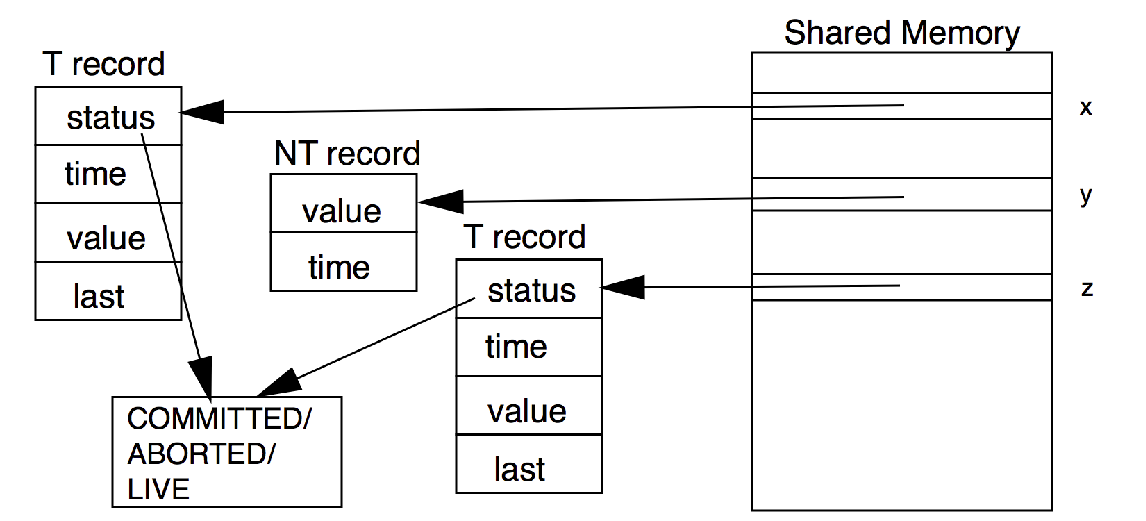
\includegraphics[width=0.6\textwidth]{SI/imgs/mem_setup_single}}
}
\caption{The memory set-up and the data structures that are used by the 
algorithm.}
\label{fig:mem_setup}
\end{figure*}

New T-records are created during the transactional write operations.
Then during
the commit operation the pointer stored at $\mathit{addr}$ is updated to point to this new T-record.
During NT-write operations new NT-records are created and the pointer at $\mathit{addr}$
is updated to point to the records.

When a read operation - be it transactional or non-transactional - accesses 
a shared variable it cannot know beforehand what type of record it will find. 
Therefore, it can be seen in the algorithm listings, that whenever 
a record is accessed, 
the operation checks its type, i.e., it checks 
whether it is a T-record or an NT-record (for example, line \ref{A02} in Fig.
\ref{fig:ntops} contains such a check. A T-record is {}``of type T'', while an 
NT-record is {}``of type NT''). 


\paragraph{T-record.}
A T-record is a structure containing the following fields.
\begin{description}
%\vspace{-0.1cm}
\item[$\mathit{status}$] This  field  indicates  the  state  of the  transaction  that  created  the
T-record. The  
state can either be LIVE, COMMITTED or ABORTED.
The state is initially set to LIVE and is not set to COMMITTED until during the commit operation when 
all locations of the transaction's write set have been set to point to the transaction's T-records
and the transaction has validated its read set.
Since a transaction can write to multiple locations, the $\mathit{status}$ field
does not directly store the state, instead it contains a
pointer to a memory location containing the state for the transaction.
Therefore the $\mathit{status}$ field of each T-record created by the same transaction will point to the same location.
This ensures that any change to the transaction's state is immediately recognized at each record.
%\vspace{-0.2cm}
\item[$\mathit{time}$] The  $\mathit{time}$  field of  a T-record  contains the  
value of  the $\mathit{GVC}$  at  the  moment the  record  was 
inserted to memory. %  into the  list of   records.
This is similar to the logical dates of TL2.
%\vspace{-0.2cm}
\item[$\mathit{value}$] This field contains the value that is meant to be written to the chosen 
memory location.
%\vspace{-0.2cm}
\item[$\mathit{last}$] During the commit operation, locations are updated to point
to the committing transaction's T-records, overwriting the previous value
that was stored in this location.
Failed validation or concurrent non-transactional operations may cause this transaction to abort 
after it updates some memory locations, but before
it fully commits.
Due to this, the previous value of the location needs to be available for future reads.
Instead of rolling back old memory values, the $\mathit{last}$ field of a T-record is used,
storing the previous value of this location.

\end{description}


\paragraph{NT-record.}
An NT-record is a structure containing the following fields.
\begin{description}
%\vspace{-0.1cm}
\item[$\mathit{value}$]
This field contains the value that is meant to be written to the chosen 
memory location.
%\vspace{-0.2cm}
\item[$\mathit{time}$]
As in the case of T-records, the $\mathit{time}$ field of NT-records 
also stores the value 
of the $\mathit{GVC}$ when the write took place.
%This field is 
%used to avoid inconsistencies %such as the ones illustrated by Figure 
%\ref{fig:timent}. 
%caused by the ABA problem.
\end{description}

Due to this different memory structure a shared lock array is no longer needed,
instead of locking each location in the write set during the commit operation, this algorithm
performs a compare and swap directly on each memory location changing the address to point to one of its T-records.
After a successful compare and swap
 and before the transactions status has been set to COMMITTED or ABORTED, the transaction effectively
owns the lock on this location.
Like in TL2, any concurrent transaction that reads the location and sees that it is locked ($\mathit{status} = $ LIVE) will
abort itself.

% During read operations (transactional or non-transactional) the additional data in these structures is used 
% to determine the most  recent valid value  of a variable.
% Should the item be of type NT-record,
% then it's $\mathit{value}$ field contains the most  
% recent valid value  of the variable. On the other hand,  should the item
%  be a  T-record, then if the $\mathit{status}$ field of
% the record is equal to COMMITTED,  
% the $\mathit{value}$ field represents the current value of the variable. Otherwise, the
% $\mathit{last}$ field contains the current value.

\paragraph{Transactional Read and Write Sets.}
Like TL2, read only transactions do not use read sets while update transactions do.
The read set is made up of a set of tuples for each location read, $\tuple{\mathit{addr, value}}$
where $\mathit{addr}$ is the address of the location read and $\mathit{value}$ is the value.
The write set is also made up of tuples for each location written by the transaction,
$\tuple{\mathit{addr, item}}$ where $\mathit{addr}$ is the location to be written
and $\mathit{item}$ is a T-record for this location.

\subsubsection{Discussion.}
One advantage of the TL2 algorithm is in its memory layout.
This is because reads and writes happen directly to memory (without indirection)
and the main amount of additional memory that is used is in the lock array.
Unfortunately this algorithm breaks that and requires an additional level of indirection
as well as additional memory per location.
While garbage collection will be required for old T- and NT-records, here we assume
automatic garbage collection such as that provided in Java, but additional solutions will be explored in future work.
These additional requirements can be an acceptable trade-off given that they are only
needed for memory that will be shared between transactions.
In the appendix of this paper we present two variations of the algorithm that trade
off different memory schemes for different costs to the transactional and
non-transactional operations.


%====================================================================

\subsection{Description of the Algorithm.}

The main goal of the algorithm is to provide strong isolation 
in such a way that  the non-transactional  operations are never blocked. 
In order  to achieve this,  the algorithm delegates most of its
concurrency   control   and  consistency   checks   to  the   transactional
code. Non-transactional  
operations access and modify  memory  locations without waiting for concurrent transactions
 and it is mainly up to transactions accessing the same location to
deal with ensuring safe concurrency.  As a
result, this algorithm gives high  priority   to non-transactional code. 

%=====================================================================
\subsection{Non-transactional Operations.}
Algorithm-specific  read  and write operations
shown in Fig. \ref{fig:ntops} must be used when a shared variable is accessed
accessed outside of a transaction.  This be done by hand or applied by a complier. 

\begin{figure}[htb]
\centering{ \fbox{
\begin{minipage}[t]{1\linewidth}%{150mm}
%\footnotesize 
\scriptsize
\renewcommand{\baselinestretch}{2.5} 
%\resetline
%\setcounter{linecounter}{200}
\begin{tabbing}
aaaaaaa\=aa\=aaaaa\=aa\=aa\=\kill %~\\


{\bf operation}  ${\sf non\_transactional\_read}(\mathit{addr})$ {\bf is}\\
\line{A01} \> $\mathit{tmp} \gets (\downarrow \mathit{addr})$; \\ 
\line{A02} \> {\bf if} $( ~\mathit{tmp}$ is of type T $ \wedge (\downarrow \mathit{tmp.status}) \neq$ COMMITTED ) \\
\line{A03}  \>\>  {\bf then if}  $(\mathit{tmp.time}  \leq \mathit{time}  \wedge  (\downarrow \mathit{tmp.status}) = $ LIVE) \\
\line{A04} \>\>\>\> {\bf then} \=${\sf \mathit{C\&S}}$($tmp.status$, LIVE, ABORTED) {\bf end if}; \\
%\line{A05} \>\> {\bf end if} \\
\line{A06} \>\>\> {\bf if} ($(\downarrow \mathit{tmp.status}) \neq $ COMMITTED)  \\
\line{A07} \>\>\>\> {\bf then} $\mathit{value} \gets \mathit{tmp.last}$ \\
\line{A08} \>\>\>\> {\bf else} $\mathit{value} \gets \mathit{tmp.value}$ \\
\line{A05} \>\>\> {\bf end if}; \\
\line{A09} \>\> {\bf else} $\mathit{value} \gets \mathit{tmp.value}$ \\
\line{A09A} \> {\bf end if}; \\
\line{A10} \> $\mathit{time} \gets {\sf max}(\mathit{time}, \mathit{tmp.time})$ \\
\line{A11} \> {\bf if} ($\mathit{time} = \infty$) {\bf then} $\mathit{time} = \mathit{GCV}$ {\bf end if}; \\
\line{A12} \> ${\sf return}$ ($\mathit{value}$) \\
{\bf end operation}. \\
\\
{\bf operation}  ${\sf non\_transactional\_write}(\mathit{addr, value})$ {\bf is}\\
\line{B01} \> allocate new variable $\mathit{next\_write}$ of type NT; \\
\line{B02} \> $\mathit{next\_write} \gets \mathit{(addr, value, \infty)}$; \\
\line{B03} \> $\mathit{addr} \gets (\uparrow \mathit{next\_write})$ \\
\line{B04} \> $\mathit{time} \gets \mathit{GVC}$; \\
\line{B05} \> $\mathit{next\_write.time} \gets \mathit{time}$; \\
{\bf end operation}.

\end{tabbing}
\normalsize
\end{minipage}
}
\caption{Non-transactional operations for reading and writing a variable.}
\label{fig:ntops}
}
\end{figure}

\paragraph{Non-transactional Read.}
The   operation  ${\sf   non\_transactional\_read()}$  is   used   to  read,
when not in a transaction, the value stored at
$\mathit{addr}$.
The  operation first  dereferences  the pointer  stored at  $\mathit{addr}$
(line \ref{A01}).
If the item is a T-record that was created by a 
transaction which  has not yet  committed then the $\mathit{value}$ field
cannot be immediately be read as the transaction might still abort.
Also if the current process has read (or written to) a value that is more recent then the transaction
(meaning the process's $\mathit{time}$ field is greater or equal to the T-records
$\mathit{time}$, line \ref{A03}) then the transaction must be directed to abort (line \ref{A04})
so that opacity and strong isolation (containment specifically) is not violated.
From a T-record with a transaction that is not committed, the value from the $\mathit{last}$
field is stored to a local variable (line \ref{A07}) and will be returned on operation completion.
Otherwise the $\mathit{value}$ field of the T- or NT-record is used (line \ref{A08}).

% Once  the correct value  has been  found  and stored  in local  variable 
% $\mathit{value}$, the local $\mathit{time}$   
% variable  is updated  (lines \ref{A10}-\ref{A11}).  The updated  $\mathit{time}$
% value is used by non-transactional operations and is necessary in order to allow 
% the detection of consistency 
% violations such as the one illustrated by Figure \ref{fig:timent}. 
% By advancing the value of $\mathit{time}$ 
% through a non-transactional read operation, 
% the serialization order of this read operation with 
% respect to transactional or non-transactional operations 
% that it read from is reflected.

Next the process local variable $\mathit{time}$ is advanced to 
the maximal 
value among its current 
value and the logical date of the T- or NT-record whose value was read.
Finally if $\mathit{time}$ was set to $\infty$ on line \ref{A10}
(meaning the T- or NT-record had yet to set its $\mathit{time}$), then it is updated
to the $\mathit{GCV}$ on line \ref{A11}.
The updated  $\mathit{time}$
value is used 
%by non-transactional operations and is necessary 
to prevent consistency 
violations. %such as the one illustrated by Figure \ref{fig:timent}. 
%caused by the ABA problem.
Once these book-keeping 
operations are finished, the local variable $\mathit{value}$
is returned (line \ref{A12}).

\paragraph{Non-transactional Write.}
The operation ${\sf non\_transactional\_write()}$ is used to write to 
a shared variable $\mathit{var}$ 
by non-transactional code.
The operation takes as input the address of the shared variable as well as the 
value to be written to it.
This operation  
creates a  new  NT-record  (line  \ref{B01}),  fills  in  its  fields  (line
\ref{B02})  and 
changes the pointer stored in $\mathit{addr}$ so that it references the 
new record it has created  (line \ref{B03}).
Unlike update transactions, non-transactional writes do not increment
the global clock variable $\mathit{GCV}$.
Instead they just read $\mathit{GCV}$ and set the NT-record's time value as well as
the process local $\mathit{time}$ to the value read (line \ref{B04} and \ref{B05}).
Since the $\mathit{GCV}$ is not incremented, several NT-records might have the same
$\mathit{time}$ value as some transaction.
When such a situation is recognized where a live transaction has the same time value
as an NT-record the transaction must be aborted (if recognized during an NT-read operation,
line \ref{A04}) or perform read set validation (if during a transactional
read operation, line \ref{C05} of Fig. \ref{fig:tops}).
This is done in order to prevent consistency violations
caused by the NT-writes not updating the $\mathit{GCV}$. %such as the one shown in Figure \ref{fig:timent}.

%==================================================================
\subsection{Transactional Read and Write Operations.}

The transactional operations for performing reads and writes are 
presented in Fig. \ref{fig:tops}. 

\paragraph{Transactional Read.}

The operation ${\sf  transactional\_read()}$ takes $\mathit{addr}$ as
input. It starts by checking  
whether the  desired variable already  exists in the  transaction{}'s write
set, in which  
case  the   value  stored there  will   be  returned  (line
\ref{C01}). If the variable is not contained  
in  the write  set, the  pointer in  $\mathit{addr}$ is  dereferenced (line
\ref{C02}) and set to $\mathit{tmp}$. Once this is detected to be a T- or NT-record
some checks are then performed in order to ensure correctness.

In the case that $\mathit{tmp}$ is a T-record the operation must check to see
if the status of the transaction for this record is still LIVE and if it is
the current transaction is aborted (line \ref{C10}).
This is similar to a transaction in TL2 aborting itself when a locked location is found.
Next the T-record's $\mathit{time}$ field is checked, and (similar to TL2) if it 
greater then the process's local $\mathit{rv}$ value the transaction must abort 
(line \ref{C12}) in order to prevent consistency violations.
If this succeeds without aborting then the local variable $\mathit{value}$
is set depending on the stats of the transaction that created the T-record (line \ref{C10}-\ref{C11}).

In case $\mathit{tmp}$ is an 
NT-record (line \ref{C03}), the operation
checks whether the value of the $\mathit{time}$ field is
greater or equal to the process local $\mathit{rv}$ value.
If it is, then this write has possibly occurred after the start of this
transaction and there are several possibilities.
In the case of an update transaction validation must be preformed, ensuring
that none of the values it has read have been updated (line \ref{C05}).
In the case of a read only transaction, the transaction
is aborted and restarted as an update transaction (line \ref{C06}).
It is restarted as an update transaction so that it has a read set that it can validate
in case this situation occurs again.
Finally local variable $\mathit{value}$ is set to be the value
of the $\mathit{value}$ field of the $\mathit{tmp}$ (line \ref{C07}).

It should be noted that the reason why the checks are performed differently
for NT-records and T-records is because the NT-write operations do not
update the global clock value while update transaction do.
This means that the checks must be more conservative in order to ensure correctness.
If performing per value validation or restarting the transaction as an update transaction
is found to be too expensive, a third possibility would be to just increment the global
clock, then restart the transaction as normal.

Finally to finish the read operation, the $\tuple{\mathit{addr, value}}$
is added to the read set if the transaction is an update transaction (line \ref{C14}),
and the value of the local variable $\mathit{value}$  is returned.

\begin{figure} [htb]
\centering{ \fbox{
\begin{minipage}[t]{1\linewidth}%{150mm}
%\footnotesize 
\scriptsize
\renewcommand{\baselinestretch}{2.5} 
%\resetline
%\setcounter{linecounter}{200}
\begin{tabbing}
aaaaaaa\=aa\=aaaaa\=aa\=aa\=\kill %~\\


{\bf operation}  ${\sf transactional\_read}(\mathit{addr})$ {\bf is}\\
\line{C01} \> {\bf if} $\mathit{addr} \in \mathit{ws}$  {\bf then} ${\sf return}$ ($\mathit{item.value}$ from $\mathit{addr}$ in $\mathit{ws}$)  {\bf end if}; \\
\line{C02} \> $\mathit{tmp} \gets (\downarrow \mathit{addr})$; \\

\line{C03} \> {\bf if} ($\mathit{tmp}$ is of type NT)   \\
\line{C04} \>\> {\bf then} {\bf if} ($\mathit{tmp.time} >= \mathit{rv}$) \\
%\> \% Do validation to prevent abort due to a non-transactional write \\
\line{C05} \>\>\> {\bf then if} this is an update transaction {\bf then} ${\sf validate\_by\_value}$() \\
\line{C06} \>\>\>\>\> {\bf else} ${\sf abort}$() and restart as an update transaction {\bf end if}; \\

\line{C06A} \>\>\> {\bf end if}; \\
\line{C07} \>\>\> $\mathit{value} \gets \mathit{tmp.value}$; \\

\line{C08} \>\> {\bf else} \\
\line{C09} \>\>\> {\bf if} ($(\mathit{status} \gets (\downarrow \mathit{tmp.status})) \neq$ COMMITTED $)$ \\
\line{C10} \>\>\>\> {\bf then if} ($\mathit{status} =$ LIVE) {\bf then} ${\sf abort}()$  {\bf else} $\mathit{value} \gets \mathit{tmp.last}$ {\bf end if}; \\
\line{C11} \>\>\>\> {\bf else} $\mathit{value} \gets \mathit{tmp.value}$ \\
\line{C11A} \>\>\> {\bf end if}; \\
\line{C12} \>\>\> {\bf if} $(\mathit{tmp.time} > \mathit{rv})$ {\bf then} ${\sf abort}()$ {\bf end if}; \\
\line{C13} \> {\bf end if}; \\

\line{C14} \> {\bf if} this is an update transaction 
                        {\bf then} add $\tuple{\mathit{addr,value}}$ to $\mathit{rs}$ {\bf end if}; \\
\line{C15} \> ${\sf return}$ ($\mathit{value}$) \\
{\bf end operation}. \\
\\
{\bf operation}  ${\sf transactional\_write}(\mathit{addr, value})$ {\bf is}\\
\line{D01} \> {\bf if} $\mathit{addr} \not\in \mathit{ws}$  \\
\line{D02} \>\> {\bf then} \> allocate a new variable $item$ of type $T$; \\
\line{D03} \>\>\> $\mathit{item}  \gets (\mathit{value, (\uparrow status), \infty})$; 
                   $\mathit{ws} \gets \mathit{ws} \cup \tuple{\mathit{addr, item}}$; \\
\line{D04} \>\> {\bf else} \> set $\mathit{item.value}$ with $\mathit{addr}$ in $\mathit{ws}$ to $\mathit{value}$ \\
\line{D05} \> {\bf end if}; \\
{\bf end operation}.
\end{tabbing}
\normalsize
\end{minipage}
}
\caption{Transactional operations for reading and writing a variable.}
\label{fig:tops}
}
\end{figure}

\paragraph{Transactional Write.}
The ${\sf transactional\_write()}$ operation
takes $\mathit{addr}$ as input value, as well as the value 
to be written to $\mathit{var}$. As  TL2, the algorithm 
performs commit-time updates of the variables it writes to. 
For this reason, the transactional write  
operation simply creates a T-record and fills in some of its 
fields (lines \ref{D02} - \ref{D03}) and 
adds it to the write set.
However, in the case that a T-record corresponding to $\mathit{addr}$  was
already present in  the write set, the
$\mathit{value}$ field of the corresponding  
T-record is simply updated (line \ref{D04}).


\paragraph{Begin and End of a Transaction} 
The operations that begin and end a transaction are ${\sf begin\_transaction()}$ 
and ${\sf try\_to\_commit()}$, presented in Fig. \ref{fig:tbc}. 
%Operation ${\sf begin\_transaction()}$ 
%initializes local variables that will be necessary 
%for the execution of the transaction.
Local variables necessary for transaction execution are initialized by  ${\sf begin\_transaction()}$.
This includes $\mathit{rv}$
which is set to $\mathit{GCV}$ and, like in TL2, is used during transactional
reads to ensure correctness, 
as well as $\mathit{status}$ which is set to LIVE and the read and write sets
which are initialized as empty sets.
(lines \ref{START1}-\ref{START3}). 

\begin{figure} [htb]
\centering{ \fbox{
\begin{minipage}[t]{1\linewidth}%{150mm}
%\footnotesize 
\scriptsize
\renewcommand{\baselinestretch}{2.5} 
%\resetline
%\setcounter{linecounter}{200}
\begin{tabbing}
aaaaaaa\=aa\=aaaaa\=aa\=aa\=\kill %~\\

{\bf operation}  ${\sf begin\_transaction}()$ {\bf is}\\
\line{START1} \> determine whether transaction is update transaction based on compiler/user input \\
\line{START2} \> $\mathit{rv} \gets \mathit{GVC}$; 
                 Allocate new variable $\mathit{status}$; \\
\line{START3} \> $\mathit{status} \gets $LIVE; \ $\mathit{ws} \gets \emptyset$; $\mathit{rs} \gets \emptyset$ \\
%\line{DA03} \> more??? \\
{\bf end operation}. \\
\\
{\bf operation}  ${\sf try\_to\_commit}()$ {\bf is}\\
\line{DA01} \> {\bf if} $(\mathit{ws} = \emptyset)$ {\bf then} ${\sf return}$ (COMMITTED) {\bf end if}; \\

\line{DA02} \> 
{\bf for each} $(\tuple{\mathit{addr, item}} \in \mathit{ws})$ {\bf do} \\

\line{DA03} \>\> $\mathit{tmp} \gets (\downarrow \mathit{addr})$; \\


\line{DA04} \>\> {\bf if} 
   ($\mathit{tmp}$ is of type $T \wedge (\mathit{status} \gets (\downarrow \mathit{tmp.status})) \neq$ COMMITTED $)$  \\
\line{DA05} \>\>\> {\bf then if} ($\mathit{status} =$ LIVE) {\bf then} ${\sf abort}()$  {\bf else} $\mathit{item.last} \gets \mathit{tmp.last}$ {\bf end if}; \\
\line{DA06} \>\>\> {\bf else} $\mathit{item.last} \gets \mathit{tmp.value}$ \\
\line{DA06A} \>\> {\bf end if}; \\
\line{DA07} \>\> $\mathit{item.time} \gets \mathit{tmp.time}$; \\

\line{DA08} \>\> {\bf if} $(\neg {\sf \mathit{C\&S}}(\mathit{addr, tmp, item}))$ {\bf then} ${\sf abort}()$ {\bf end if}; \\
%\line{DA09} \>\>\> {\bf then} ${\sf abort}()$ \\
%\line{DA10} \>\> {\bf end if} \\

\line{DA11} \> {\bf end for}; \\

\line{DA12} \> $\mathit{time} \gets {\sf fetch\&increment}(\mathit{GVC})$; ${\sf validate\_by\_value}()$; \\

%\line{DA13} \> ${\sf validate\_by\_value}()$;  \\


%\> \% Ensure the writes haven't been overwritten by non-transactional writes \\
\line{DA14} \> 
{\bf for each} ($\tuple{\mathit{addr, item}} \in \mathit{ws}$) {\bf do} \\
\line{DA15} \>\> $\mathit{item.time} \gets \mathit{time}$; \\
\line{DA16} \>\> {\bf if} $(\mathit{item} \neq (\downarrow \mathit{addr}))$  
                 {\bf then}  
                   ${\sf abort}()$ 
                {\bf end if}; \\

\line{DA17} \> {\bf end for}; \\
\line{DA18} \> {\bf if} ${\sf \mathit{C\&S}}$($\mathit{status}$, LIVE, COMMITTED) \\
\line{DA19} \>\> {\bf then} \> ${\sf return}$ (COMMITTED)\\
\line{DA20} \> \> {\bf else} \= ${\sf abort}()$ \\
\line{DA21} \> {\bf end if};  \\
{\bf end operation}.

\end{tabbing}
\normalsize
\end{minipage}
}
\caption{Transaction begin/commit.}
\label{fig:tbc}
}
\end{figure}

After  performing all  required read  and write  operations,  a transaction
tries to commit, using the operation  ${\sf try\_to\_commit()}$.
Similar to TL2, a ${\sf try\_to\_commit()}$ operation 
starts by trivially committing if the transaction was a read-only one 
(line \ref{DA01}) while
an update transaction must announce to concurrent operations what locations it will be updating
(the items in the write set).
However, the algorithm  differs 
here from TL2, given that 
it is faced with concurrent non-transactional operations
that do not rely on locks and never block. 
This implies 
that even after acquiring the locks for all items in its write set, 
a transaction could be {}``outrun'' by 
a non-transactional operation that writes to one of those items
causing the transaction to be required to abort in order to ensure correctness. 
As described previously, while TL2 locks items in its write set using a
lock array, this algorithm compare and swaps pointers directly to the T-records
in its write set (lines \ref{DA02}-\ref{DA11}) while keeping a reference to the previous value.
The previous value is stored in the T-record before the compare and swap is performed (lines \ref{DA05}-\ref{DA06})
with a failed compare and swap resulting in the abort of the transaction.
If while performing these compare and swaps the transaction notices
that another LIVE transaction is updating this memory, it aborts itself
(line \ref{DA05}).
By using these T-records instead of locks concurrent operations have access to necessary metadata
used to ensure correctness.

The operation then advances the $\mathit{GVC}$, taking the
new value of the clock as the logical time for this transaction (line \ref{DA12}).
Following this, the read set of the transaction is validated for
correctness  (line \ref{DA12}). %was: (line \ref{DA13}).
Once validation has been performed the operation must
ensure that non of its writes have been concurrently
overwritten by non-transactional operations (lines \ref{DA14}-\ref{DA17})
if so then the transaction must abort in order to (line \ref{DA16}) to ensure consistency.
During this check the transaction updates the $\mathit{time}$
value of its T-records to the transactions logical time (line \ref{DA15})
similar to the way TL2 stores time values in the lock array
so that future operations will know the serialization of this transaction's updates.

Finally the
transaction can mark its updates as valid by 
changing its 
$\mathit{status}$ variable from LIVE to COMMITTED (line \ref{DA18}).
This is done using a compare and swap as there could be
a concurrent non-transactional operations trying to abort the transaction.  
If this succeeds then the transaction has successfully committed, otherwise
it must abort and restart.


\begin{figure} [htb]
\centering{ \fbox{
\begin{minipage}[t]{1\linewidth}%{150mm}
%\footnotesize 
\scriptsize
\renewcommand{\baselinestretch}{2.5} 
%\resetline
%\setcounter{linecounter}{200}
\begin{tabbing}
aaaaaaa\=aa\=aaaaa\=aa\=aa\=\kill %~\\

{\bf operation} ${\sf validate\_by\_value}()$ {\bf is}\\
\line{H01} \> $\mathit{rv} \gets \mathit{GVC}$; \\
\line{H02} \> {\bf for each} $\tuple{\mathit{addr, value}}$ in $\mathit{rs}$ {\bf do} \\
\line{H03} \>\> $\mathit{tmp} \gets (\downarrow \mathit{addr})$; \\
\line{H04} \>\> {\bf if} ($\mathit{tmp}$ is of type T $ \wedge \mathit{tmp.status} \neq $ COMMITTED) \\
\line{H05} \>\>\> {\bf then if} ($\mathit{tmp.status} =$ LIVE $\wedge \mathit{item} \not \in \mathit{ws}$)
     {\bf then} ${\sf abort}()$ {\bf end if}; \\
\line{H06} \>\>\>\> $\mathit{new\_value} \gets \mathit{tmp.last}$; \\
\line{H07} \>\>\> {\bf else} $\mathit{new\_value} \gets \mathit{tmp.value}$ \\
\line{H07A} \>\> {\bf end if}; \\
\line{H08} \>\> {\bf if} $\mathit{new\_value} \neq \mathit{value}$
     {\bf then} ${\sf abort}()$ {\bf end if}; \\
\line{H09} \> {\bf end for}; \\
{\bf end operation}. \\
\\
{\bf operation} ${\sf abort}()$ {\bf is}\\
\line{AB01} \> $\mathit{status} \gets $ ABORTED; \\
\line{AB02} \> the transaction is aborted and restarted \\
%\line{H21} \> free items in $\mathit{ws}$, $\mathit{rs}$, and $\mathit{ntrs}$; \\
%\line{H22} \> jump to line \ref{START1} \\
{\bf end operation}. \\
\end{tabbing}
\normalsize
\end{minipage}
}
\caption{Transactional helper operations.}
\label{fig:helpers}
}
\end{figure}


\paragraph{Transactional Helping Operations.} 
Apart from the basic operations for starting, committing, 
reading and writing, a transaction makes use of helper 
operations to perform aborts and validate the read set.
 Pseudo-code for this kind of helper operations 
is given in Fig. \ref{fig:helpers}.

Operation ${\sf validate\_by\_value()}$ is an operation that performs 
validation of the read set of a transaction. 
Validation fails 
if any location in $\mathit{rs}$ is 
currently being updated by another transaction (line \ref{H05})
or has had its changed since it was first read by the transaction (line \ref{H08})
otherwise it succeeds.
The transaction is immediately aborted if validation fails (lines \ref{H05}, \ref{H08}).
Before the validation is performed the local variable $\mathit{rv}$ is updated
to be the current value of $\mathit{GVC}$ (line \ref{H01}).
This is done because if validation succeeds then transaction is valid at this time
with a larger
clock value possibly preventing future validations and aborts.

When a transaction is aborted in the present algorithm, 
the status of the current transaction is set to ABORTED (line \ref{AB01}) and
it is immediately restarted as a new transaction.

%========================================================================

\section{Conclusion}
\label{sec:conclusions}
This paper has presented an algorithm that achieves non-blocking strong 
isolation  ``on top of'' a TM algorithm based on logical dates and locks, 
namely  TL2. 
In the case of a conflict between a transactional and a non-transactional
operation, this algorithm gives priority to 
the non-transactional operation, 
with the reasoning that while an eventual abort or restart is part of the 
specification of a transaction,
this is not the case for a single shared read or write operation. 
Due to this priority mechanism, 
the proposed algorithm is   particularly appropriate  for environments 
in which processes do not rely heavily
on the use of especially large transactions along with non-transactional write operations.
In such environments, terminating strong isolation is  provided for transactions, 
while conventional read and write operations execute with a small additional overhead.


%\section{Refernces}\label{references}

% \begin{thebibliography}{4}

% \bibitem{afek10}
%  Afek, Y.,  Avni, H.,   Dice, D.,  Shavit, N.: Efficient lock free privatization. 
% In: {\it Proc.  14th Int'l conference on Principles of Distributed Systems 
% (OPODIS'10)}, pp. 333--347, Springer-Verlag,  LNCS \#6490 (2010) 
% 
% \bibitem{CIR12} 
% Crain, T., Imbs, D.,  Raynal, M.: 
% Towards a Universal Construction for Transaction-based Multiprocess Programs.
% In: {\it Proc. 13th Int'l Conference on Distributed Computing and Networking (ICDCN'12)}, 
% pp. 61--75, Springer Verlag LNCS \#7129 (2012) 
% 
% \bibitem{DS09}
% Dalessandro, L., Scott, M.:
% Strong Isolation is a Weak Idea. 
% In: {\it Proc. Workshop on transactional memory (TRANSACT'09)} (2009)
% 
% \bibitem{dice10}
% Dice, D., Matveev, A.,  Shavit, N.:
% Implicit privatization using private transactions. 
% In: {\it Proc. Workshop on transactional memory (TRANSACT'10)} (2010)
% 
% \bibitem{dice06}
% Dice, D., Shalev O., Shavit, N.:
% Transactional Locking II.
% In: {\em Proc. 20th Int'l Symp. on Distributed Computing (DISC'06)},
% Springer-Verlag, LNCS \#4167, pp.~194--208 (2006)
% 
% \bibitem{guerraoui08}
% Guerraoui, R., Kapalka, M.:  On the correctness of transactional memory. 
% In: {\it  Proc. 13th ACM SIGPLAN Symposium on Principles and Practice of 
% Parallel Programming (PPoPP '08)},  ACM Press, pp.  175--184 (2008)
% 
% \bibitem{harris06}
%  Harris, T.,  Larus, J.,  Rajwar, R.:
% Transactional Memory, 
% {\it 2nd edition, Synthesis Lectures on Computer Architecture},
% Morgan \& Claypool Publishers (2006)
% 
% \bibitem{herlihy93}
% Herlihy, M., Moss J.M.B.: Transactional memory: architectural support for lock-free data structures, 
% In: {\it Proc.  of the 20th annual Int'l Symposium on Computer Architecture 
% (ISCA '93)}, ACM Press, pp. 289--300 (1993)
% 
% \bibitem{IR09} 
% Imbs, D., Raynal, M.: 
% A versatile   STM protocol with invisible read operations 
% that satisfies  the  virtual world consistency condition.
% In: {\it   16th  Colloquium   on  Structural   Information   and  Communication Complexity  (SIROCCO'09)}, 
% Springer Verlag LNCS   \#5869, pp. 266--280 (2009)
% 
% \bibitem{ma07}
%  Maessen, J.-W., Arvind, M.:
%  Store Atomicity for Transactional Memory. 
% {\it Electronic  Notes  on Theoretical  Computer Science}, 
% 174(9):117--137 (2007).
% 
% \bibitem{blundell06}
%  Martin, M.,  Blundell, C., Lewis, E.:
%  Subtleties of Transactional Memory Atomicity Semantics. 
% {\it IEEE Computer Architecture  Letters},  5(2):  (2006)
% 
% \bibitem{MS12}
% Matveev, A.,  Shavit, N.:
% Towards a Fully Pessimistic STM Model. 
% In: {\it Proc. Workshop on transactional memory (TRANSACT'12)} (2012)
% 
% \bibitem{MTCM07}
% Minh, C., Trautmann, M., Chung, J., McDonald, A., Bronson, N., Casper, J., Kozyrakis, C., Olukotun, K.:
% An effective hybrid transactional memory system with strong isolation guarantees.
% In: {\it SIGARCH Comput. Archit. News}, 35(2):69--80 (2007)
% 
% \bibitem{P79}
% Papadimitriou, Ch.H.:
% The Serializability of Concurrent Updates. 
% {\it Journal of the ACM},  26(4):631--653 (1979) 
% 
% \bibitem{SMSA08}
%  Schneider, F., Menon, V., Shpeisman, T., Adl-Tabatabai, A.:
%  Dynamic optimization for efficient strong atomicity.
% In: {\it ACM  SIGPLAN Noticers}, 43(10):181--194  (2008)
% 
% \bibitem{scott07}
%  Scott, M.L.,  Spear, M.F., Dalessandro, L.,   Marathe, V.J.:
%  Delaunay Triangulation with Transactions and Barriers. 
% In: {\it Proc.  10th IEEE Int'l Symposium on Workload Characterization (IISWC '07)},
%  IEEE Computer Society, pp. 107--113 (2007)
% 
% \bibitem{shavit95}
%  Shavit, N., Touitou, D.: Software transactional memory. 
% Software Transactional Memory. 
% In: {\it Distributed  Computing}, 10(2):99--116 (1997) 
% 
% \bibitem{shpeis07}
%  Shpeisman, T.,  Menon, V.,  Adl-Tabatabai, A.R.,  Balensiefer, S.,  Grossman, D.,
%  Hudson, R.L., Moore, K.F., Saha, B.:
% Enforcing isolation and ordering in STM. 
% In: {\it ACM  SIGPLAN Noticers}, 42(6):78--88  (2007)
% 
% \bibitem{spear08}
% Spear M.F.,  Dalessandro L.,  Marathe V.J.,  Scott, M.L.:
% Ordering-Based Semantics for Software Transactional Memory. 
% In: {\it Proc  12th Int'l Conf. on Principles of Distributed Systems 
% (OPODIS '08)},  Springer-Verlag LNCS \#5401, pp. 275--294 (2008) 
% 
% \bibitem{spear07}
% Spear, M.F.,  Marathe, V.J.,  Dalessandro, L.,  Scott, M.L.: 
% Privatization techniques for software transactional memory. 
% In: {\it Proc. 26th  annual ACM symposium on Principles of Distributed Computing 
% (PODC '07)}, . ACM press, pp.  338--339, (2007)


% \end{thebibliography}



% \begin{appendix}\label{sec:appendix}



\section{Version of algorithm that does not use NT-records}
This algorithm also provides wait-free NT read and write operations.
The difference is that NT-records are not used.
Instead NT values are read and written directly from memory.
By doing this, memory allocations are not needed in NT writes and NT reads have
one less level of indirection.

The cost of this is more frequent validations required in transactions when conflicts with NT writes occur.
This algorithm is shown in Figs. \ref{fig:ntops2}-\ref{fig:tbc2}.


\begin{figure}[htb]
\centering{ \fbox{
\begin{minipage}[t]{150mm}
\footnotesize 
\renewcommand{\baselinestretch}{2.5} 
%\resetline
%\setcounter{linecounter}{200}
\begin{tabbing}
aaaaaaa\=aa\=aaaaa\=aa\=aa\=\kill %~\\


{\bf operation}  ${\sf non\_transactional\_read}(\mathit{addr})$ {\bf is}\\
\line{MA01} \> $\mathit{tmp} \gets (\downarrow \mathit{addr})$; \\ 
\line{MA02} \> {\bf if} $( ~\mathit{tmp}$ is of type T )  \\
\line{MA03}  \>\>  {\bf then if}  ($\mathit{tmp.status} = $ LIVE) \\
\line{MA04} \>\>\>\> {\bf then} \=${\sf \mathit{C\&S}}$($tmp.status$, LIVE, ABORTED) \\
\line{MA05} \>\>\> {\bf end if}; \\
\line{MA06} \>\>\> {\bf if} ($tmp.status = $ ABORTED) \\
\line{MA07} \>\>\>\> {\bf then} $\mathit{value} \gets \mathit{tmp.last}$ \\
\line{MA08} \>\>\>\> {\bf else} $\mathit{value} \gets \mathit{tmp.value}$ \\
\line{MA09} \>\>\> {\bf end if}; \\
\line{MA10} \>\> {\bf else} $\mathit{value} \gets \mathit{tmp}$ \\
\line{MA10A} \> {\bf end if}; \\
\line{MA11} \> ${\sf return}$ $(\mathit{value})$ \\
{\bf end operation}. \\
\\
{\bf operation}  ${\sf non\_transactional\_write}(\mathit{addr, value})$ {\bf is}\\
\line{MB01} \> $\mathit{addr} \gets (\uparrow \sf{unMark}(\mathit{value}))$
{\bf end operation}.

\end{tabbing}
\normalsize
\end{minipage}
}
\caption{Non-transactional operations for reading and writing a variable.}
\label{fig:ntops2}
}
\end{figure}











\begin{figure} %[htb]
\centering{ \fbox{
\begin{minipage}[t]{150mm}
\footnotesize 
\renewcommand{\baselinestretch}{2.5} 
%\resetline
%\setcounter{linecounter}{200}
\begin{tabbing}
aaaaaaa\=aa\=aaaaa\=aa\=aa\=\kill %~\\


{\bf operation}  ${\sf transactional\_read}(\mathit{addr})$ {\bf is}\\
\line{MC01} \> {\bf if} $\mathit{addr} \in \mathit{ws}$  {\bf then} ${\sf return}$ ($\mathit{item.value}$ from $\mathit{addr}$ in $\mathit{ws}$)  {\bf end if}; \\
\line{MC02} \> $\mathit{tmp} \gets (\downarrow \mathit{addr})$; \\
\line{MC03} \> {\bf if} 
   ($\mathit{tmp}$ is of type $T$ ) \\
\line{MC04} \>\> {\bf then if} ($\mathit{status} =$ LIVE) {\bf then} ${\sf abort}$() {\bf end if}; \\
\line{MC05} \>\>\> {\bf if} $(\mathit{tmp.time} > \mathit{rv})$ {\bf then} ${\sf abort}$() {\bf end if}; \\
\line{MC06} \>\>\> {\bf if} ($\mathit{status} =$ COMMITTED)   \\
\line{MC07} \>\>\>\> {\bf then} $\mathit{value} \gets \mathit{tmp.val}$ \\
\line{MC08} \>\>\>\> {\bf else} $\mathit{value} \gets \mathit{tmp.last}$ \\
\line{MC08A} \>\>\> {\bf end if}; \\
\line{MC09} \>\> {\bf else} \\
\> \% Do validation to prevent abort due to a non-transactional write \\
\line{MC10} \>\>\> $\mathit{rv} \gets {\sf validate\_by\_value}()$; \\
\line{MC11} \>\>\> $\mathit{value} \gets \mathit{tmp}$; \\
\line{MC12} \> {\bf end if}; \\
\line{MC13} \> {\bf if} this is an update transaction {\bf then} add $\mathit{value}$ to $\mathit{rs}$ {\bf end if}; \\
\line{MC14} \> ${\sf return}$ $(\mathit{value})$ \\

{\bf end operation}. \\
\\
{\bf operation}  ${\sf transactional\_write}(\mathit{addr, value})$ {\bf is}\\
\line{MD01} \> {\bf if} $\mathit{addr} \not\in \mathit{ws}$  \\
\line{MD02} \>\> {\bf then} \> allocate a new variable $item$ of type $T$; \\
\line{MD03} \>\>\> $\mathit{item}  \gets (\mathit{addr, value, status, \infty})$; 
                   $\mathit{ws} \gets \mathit{ws} \cup \mathit{item}$ \\
\line{MD04} \>\> {\bf else} \> set $\mathit{item.value}$ with $\mathit{addr}$ in $\mathit{ws}$ to $\mathit{value}$ \\
\line{MD05} \> {\bf end if} \\
{\bf end operation}.
\end{tabbing}
\normalsize
\end{minipage}
}
\caption{Transactional operations for reading and writing a variable.}
\label{fig:tops2}
}
\end{figure}







\begin{figure} [htb]
\centering{ \fbox{
\begin{minipage}[t]{150mm}
\footnotesize 
\renewcommand{\baselinestretch}{2.5} 
%\resetline
%\setcounter{linecounter}{200}
\begin{tabbing}
aaaaaaa\=aa\=aaaaa\=aa\=aa\=\kill %~\\

{\bf operation}  ${\sf try\_to\_commit}()$ {\bf is}\\
\line{MDA01} \> {\bf if} $(\mathit{ws} = \emptyset)$ {\bf then} ${\sf return}$ (COMMITTED) {\bf end if}; \\

\line{MDA02} \> 
{\bf for each} $(\mathit{item} \in \mathit{ws})$ {\bf do} \\

\line{MDA03} \>\> $\mathit{tmp} \gets (\downarrow \mathit{addr})$; \\


\line{MDA04} \>\> {\bf if} 
   ($\mathit{tmp}$ is of type $T$) \\
\line{MDA05} \>\>\> {\bf then if} (($\mathit{status} \gets \mathit{tmp.status}$) $=$ COMMITTED) \\
\line{MDA05A} \>\>\>\>\> {\bf then} $\mathit{item.last} \gets \mathit{tmp.value}$ \\
\line{MDA06} \>\>\>\>\> {\bf else if} ($\mathit{status} =$ ABORTED) {\bf then} $\mathit{item.last} \gets \mathit{tmp.last}$ \\
\line{MDA07} \>\>\>\>\> {\bf else} ${\sf abort}()$ \\
\line{MDA07A} \>\>\>\> {\bf end if}; \\
\line{MDA08} \>\>\> {\bf else} $\mathit{item.last} \gets \mathit{tmp}$ \\
\line{MDA08A} \>\> {\bf end if}; \\

\line{MDA09} \>\> {\bf if} $(\neg {\sf \mathit{C\&S}}(\mathit{item.addr, tmp, item}))$ {\bf then} ${\sf abort}()$ {\bf end if}; \\
%\line{MDA10} \>\>\> {\bf then} ${\sf abort}()$ \\
%\line{MDA11} \>\> {\bf end if}; \\

\line{MDA12} \> {\bf end for}; \\

\line{MDA13} \> $\mathit{time} \gets {\sf fetch\&increment}(\mathit{GVC})$; \\

\line{MDA14} \> ${\sf validate\_by\_value}$(); \\


\> \% Ensure the writes haven't been overwritten by non-transactional writes \\
\line{MDA15} \> 
{\bf for each} $(\mathit{item} \in \mathit{ws})$ {\bf do} \\

\line{MDA16} \>\> {\bf if} $(\mathit{item} \neq (\downarrow \mathit{item.addr}))$  
                 {\bf then} 
                   ${\sf abort}()$ 
                {\bf end if} \\
\line{MDA17} \>\> $\mathit{item.time} \gets \mathit{time}$; \\
\line{MDA18} \> {\bf end for}; \\
\line{MDA19} \> {\bf if} (${\sf \mathit{C\&S}}$($\mathit{status}$, LIVE, COMMITTED)) \\
\line{MDA20} \>\> {\bf then} \> ${\sf return}$ (COMMITTED)\\
\line{MDA21} \> \> {\bf else} \= ${\sf abort}()$ \\
\line{MDA22} \> {\bf end if};  \\
{\bf end operation}.

\end{tabbing}
\normalsize
\end{minipage}
}
\caption{Transaction commit.}
\label{fig:tbc2}
}
\end{figure}



\begin{figure}[htb]
\centering{ \fbox{
\begin{minipage}[t]{150mm}
\footnotesize 
\renewcommand{\baselinestretch}{2.5} 
%\resetline
%\setcounter{linecounter}{200}
\begin{tabbing}
aaaaaaa\=aa\=aaaaa\=aa\=aa\=\kill %~\\


{\bf operation}  ${\sf non\_transactional\_read}(\mathit{addr})$ {\bf is}\\
\line{N01} \> $\mathit{lock} \gets {\sf load\_lock}(\mathit{addr})$; \\ 
\line{N02} \> $\mathit{value} \gets (\downarrow \mathit{addr})$; \\ 
\line{N03} \> {\bf if} ($~\mathit{lock}$ is locked  $\wedge \mathit{tmp.status} = $ COMMITTED $\wedge \mathit{addr} \in \mathit{lock.ws}$) \\
\line{N04} \>\> {\bf then} $\mathit{value} \gets \mathit{item.value}$ from $\mathit{addr}$ in $\mathit{lock.ws}$ \\
\line{N05} \> {\bf end if}; \\

\line{N06} \> ${\sf return}$ $(\mathit{value})$ \\
{\bf end operation}. \\
\\
{\bf operation}  ${\sf non\_transactional\_write}(\mathit{addr, value})$ {\bf is}\\
\line{NB01} \> Perform a transactional begin/write/commit operation \\
{\bf end operation}.

\end{tabbing}
\normalsize
\end{minipage}
}
\caption{Non-transactional operations for reading and writing a variable.}
\label{fig:noblock-readonly}
}
\end{figure}


\section{Version of algorithm with non-blocking NT-reads and blocking NT-writes}

This algorithm allows wait-free NT read operations.
The only change that is needed to the base TL2 algorithm is that when an item is locked it points to the write-set of the transaction, and that each
transaction has a marker that is initialized as $\mathit{LIVE}$ and is set to $\mathit{COMMITTED}$ just before the transaction starts performing write backs 
during the commit phase.
The NT-read operation is shown in Fig. \ref{fig:noblock-readonly}.

% \end{appendix}
% 
% \end{document}